\documentclass[12pt,a4paper]{article}
\usepackage[utf8]{inputenc}
\usepackage[hidelinks]{hyperref}
\usepackage[swedish]{babel}
\usepackage[T1]{fontenc}
\usepackage[parfill]{parskip} 
\usepackage[a4paper, total={6in,8in}]{geometry}
\usepackage{mathtools,graphicx,url,amsmath, tikz, csquotes, biblatex, upgreek, newtxtext, newtxmath, tcolorbox, wrapfig, physics}

% Gör en mapp som heter bilder och lägg sedan in alla bilder där för att använda nedan.
\graphicspath{{./bilder/}}

% Numrera i varje sektion, kommentera ut för att bli av med det.
%\numberwithin{equation}{section}
%\numberwithin{figure}{section}
\newcounter{excount}
\counterwithin{excount}{section}
\setcounter{excount}{0}

%annat
%\newcommand{\abs}[1]{\left\lvert #1 \right\rvert }
\newcommand{\unit}[1]{\textrm{ #1}}
\newcommand{\der}[2]{\frac{d#1}{d#2}}
\newcommand{\pd}[2]{\frac{\partial #1}{\partial #2}}
\newcommand{\sgn}{\, \textrm{sgn}}

%enhetsvektorer
\newcommand{\iunit}{\, \hat{i}}
\newcommand{\junit}{\, \hat{j}}
\newcommand{\kunit}{\, \hat{k}}

%lådor för definition, exempel och notering.
\newcommand{\exempel}[2]{
    \begin{tcolorbox}[colback=white,colframe=blue!80,coltitle=white,title={Exempel \stepcounter{excount} \theexcount : #1}]
        #2
    \end{tcolorbox}
}
\newcommand{\notera}[1]{
    \begin{tcolorbox}[colback=red!5!white,colframe=red!75,coltitle=white,title= Notera att:]
        #1
    \end{tcolorbox}
}
\newcommand{\defin}[2]{
    \begin{tcolorbox}[colback=yellow!5!white,colframe=yellow!100,coltitle=black,title= Definition: #1]
        #2
    \end{tcolorbox}
}
\newcommand{\sats}[2]{
    \begin{tcolorbox}[colback=green!5!white,colframe=green!75,coltitle=black,title= Sats: #1]
        #2
    \end{tcolorbox}
}

%figurer, använda bara vanliga lol detta var inte värt det
\newcommand{\figil}[2]{
    \begin{center}
        \includegraphics[width=#1\textwidth]{#2}
    \end{center}
}
\newcommand{\figfl}[5]{
    \begin{figure}[#1]
        \centering
        \includegraphics[width=#2\textwidth]{#3}
        \caption{#4}
        \label{fig:#5}
    \end{figure}
}
\newcommand{\wf}[5]{
    \begin{wrapfigure}{#1}{#2\textwidth}
        \includegraphics[width=#2\textwidth]{#3}
        \caption{#4}
        \label{fig:#5}
    \end{wrapfigure}}

% kommentera ut för att använda.
\addbibresource{referenser.bib}

\title{Mekanik III - Labbrapport}
\author{Erik Björk, Jakob Dahlgren}
\date{\today}

\begin{document}
\maketitle
\clearpage

\tableofcontents

\begin{abstract}
    blah
\end{abstract}

\section{Inledning}
Laborationen undersökte kopplade svängningar hos två pendlar, med en fjäder emellan.
\section{Teori}

\section{Metod}
\subsection{Materiel}
\begin{itemize}
    \item Stång med massa
    \item Fjäder
    \item Vinkelgivare, kopplad till mätprogram (2 st)
\end{itemize}

\subsection{Utförande}
Stängerna med massor hängdes upp i vinkelgivare. En fjäder sattes fast mellan stängerna. Mätprogrammet statades, och de teoretiskt härledda egenmoderna togs fram. Under laborationen använder PASCO \emph{Capstone}.

Massorna positionerades motsvarigt till varje randvillkor, och systemets rörelse mättes. Experimentet upprepades flera gånger för varje randvillkor för att använda den mest representativa mätserien.

Efter mätningarna gjordes kurvanpassningar till mätdatan för att hitta systemets egenfrekvenser. Dessa jämfördes med den teoretiskt beräknade värdenna, baserat på mätningar av pendelns tröghetsmoment, massa och fjäderkonstanten.
\section{Resultat}

\subsection{Experimentkörning}
I figurerna \ref{fig:A},\ref{fig:B},\ref{fig:C} syns datan för de första fem sekundrarna av mätningar. Där är båda pendlarna med, som $\theta$ och $\phi$, samt egenmoderna $q_1,q_2$.

\begin{figure}[htbp]
    \centering
    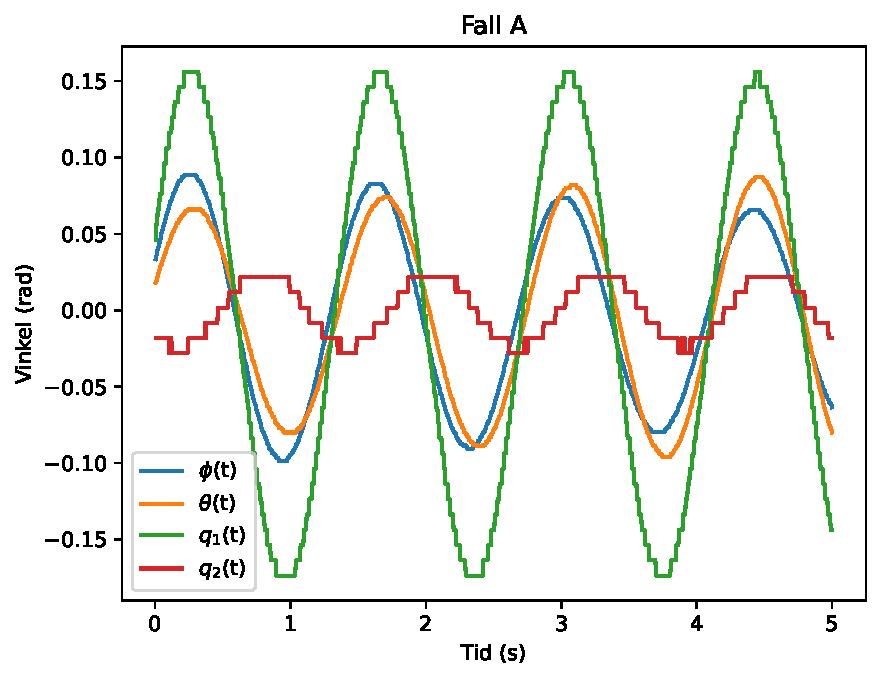
\includegraphics[width=0.7\textwidth]{plot_A.pdf}
    \caption{Mätdata från fall A.}
    \label{fig:A}
\end{figure}

\begin{figure}[htbp]
    \centering
    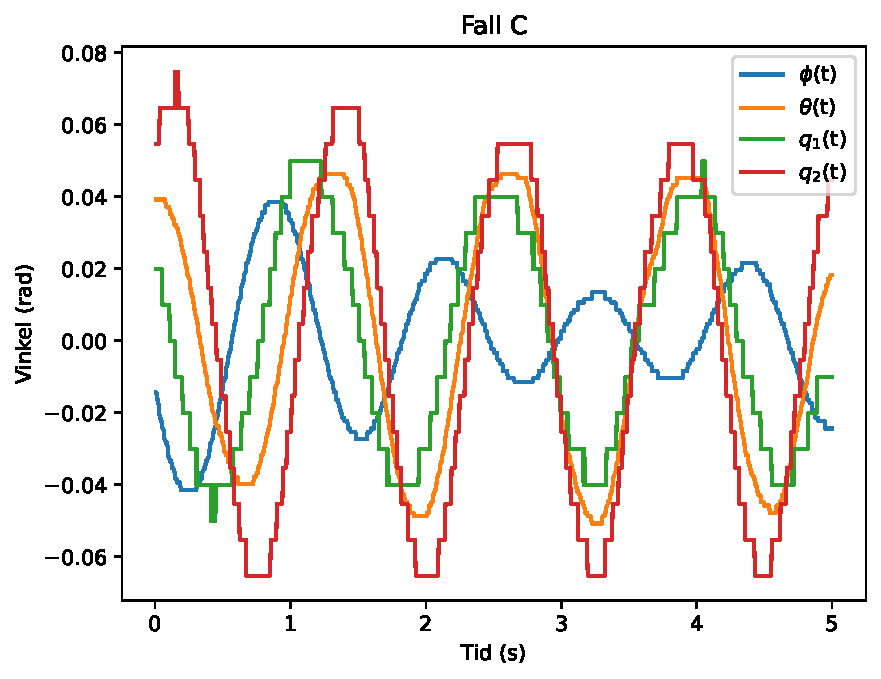
\includegraphics[width=0.7\textwidth]{plot_C.pdf}
    \caption{Mätdata från fall C.}
    \label{fig:B}
\end{figure}

\begin{figure}[htbp]
    \centering
    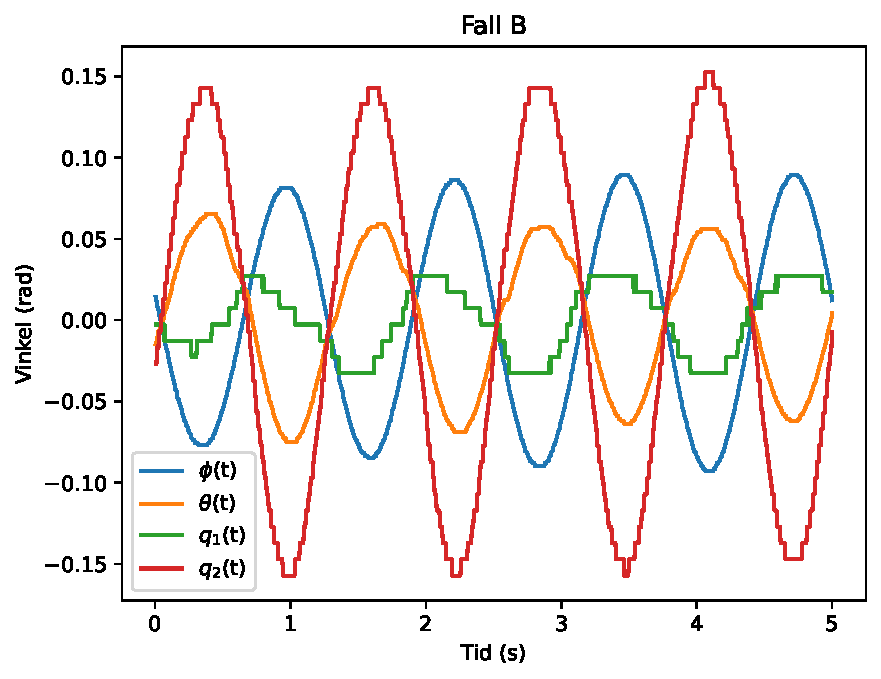
\includegraphics[width=0.7\textwidth]{plot_B.pdf}
    \caption{Mätdata från fall C.}
    \label{fig:C}
\end{figure}

Från en sinusanpassning i \emph{Capstone} fick man ut egenfrekvenserna för vardera fall:
\begin{align}
    \begin{cases}
        \omega_{A1} &= 4.52\unit{rad/s}\\
        \omega_{B1} &= 4.52\unit{rad/s}\\
        \omega_{C1} &= 4.53\unit{rad/s}
    \end{cases},\quad 
    \begin{cases}
        \omega_{A2} &= 5.05\unit{rad/s}\\
        \omega_{A2} &= 5.06\unit{rad/s}\\
        \omega_{A2} &= 5.06\unit{rad/s}
    \end{cases} \label{eq: omega cap}
\end{align}

\subsection{Mätningar}
lägg in alla mätningar med osäkerheter här!!!!!
\include{diskussion}
\include{slutsats}
\printbibliography
\appendix
%\include{härledning}
\end{document}
